\documentclass[pdftex,12pt,xcolor=svgnames]{beamer}

\mode<presentation>
{
  \usetheme{boxes}
  \usecolortheme[named=MidnightBlue]{structure}
  %\setbeamercolor{normal text}{bg=NavajoWhite!20}
  %% \usefonttheme{serif}
  \setbeamertemplate{navigation symbols}{}
  % Show frame number and author name in footline
  \setbeamertemplate{frametitle}[default][center]
  \setbeamertemplate{footline}[frame number]
  \setbeamertemplate{items}[circle]
  %\addtobeamertemplate{footline}{\quad\textcolor{gray}{James Robert Lloyd}}{}
  % Set frame titles in small capitals
  %% \setbeamerfont{frametitle}{shape=\scshape,family=\rmfamily,size={\fontsize{16}{20}}}
  %% \setbeamercolor{frametitle}{bg=gray!60!white,fg=black}
  %% \setbeamercolor{frametitle}{bg=blue,fg=black}
  % Alerted text: blue (uncomment second line if theme sets alerted text to bold)
  \setbeamercolor{alerted text}{fg=blue}
  %\setbeamerfont*{alerted text}{}
  \setbeamertemplate{bibliography item}[text] %{\hbox{\donotcoloroutermaths$\blacktriangleright$}}
  \setbeamertemplate{bibliography entry title}{}
  \setbeamertemplate{bibliography entry author}{}
  \setbeamertemplate{bibliography entry note}{}
  \setbeamertemplate{bibliography entry location}{}

}
\usepackage[english]{babel}
\usepackage[latin1]{inputenc}
\usepackage{times}
\usepackage[T1]{fontenc}
\usepackage{hyperref}
\usepackage{multimedia}
\usepackage{eepic}
\usepackage{graphicx}
%\usepackage[nohug]{latexinclude/diagrams}
\usepackage{tikz}
\usetikzlibrary{calc}

%% \newcommand{\footlineextra}[1]{
%%     \begin{tikzpicture}[remember picture,overlay]
%%         \node[yshift=1.5ex,anchor=south east] at (current page.south east)
%% {#1};
%%     \end{tikzpicture}
%% }

\newcommand{\footlineextra}[1]{
    \begin{tikzpicture}[remember picture,overlay]
        \node[xshift=-5ex,yshift=-0.5ex,anchor=south east] at (current page.south east)
             {\mbox{\tiny \textcolor{MidnightBlue}{#1}}};
    \end{tikzpicture}
}

\def\sectionframe#1{
  {
    \setbeamertemplate{footline}{\empty}
    \begin{frame}{}
      \begin{center}
        \huge\sc #1
      \end{center}
    \end{frame}
  }
}


\usepackage{etex}
\usepackage{tabularx}
\usepackage{include/picins}
%\usepackage{include/preamble}
\usepackage{setspace}
\usepackage{xcolor}
\usepackage{tikz}
\usepackage{listings}
\usepackage[noend]{algpseudocode}
\usepackage{algorithm}
\usepackage{caption}
\usepackage{array}
\usepackage{booktabs}

% Math typesetting.
\newcommand{\vx}{\mathbf{x}}
\newcommand{\vX}{\mathbf{X}}
\newcommand{\vw}{\mathbf{w}}
\newcommand{\vv}{\mathbf{v}}
\newcommand{\vr}{\mathbf{r}}
\newcommand{\vg}{\mathbf{g}}
\newcommand{\vI}{\mathbf{I}}
\newcommand{\vzero}{\bf{0}}
\newcommand{\ones}[1]{\mat{1}_{#1}}
\newcommand{\eye}[1]{\mat{E}_{#1}}
\newcommand{\tra}{^{\mathsf{T}}}
\newcommand{\vect}[1]{{\bf{#1}}}
\newcommand{\mat}[1]{\mathbf{#1}}
\newcommand{\pderiv}[2]{\frac{\partial #1}{\partial #2}}
\newcommand{\npderiv}[2]{\nicefrac{\partial #1}{\partial #2}}
\newcommand{\argmin}{\operatornamewithlimits{argmin}}
\newcommand{\argmax}{\operatornamewithlimits{argmax}}
\newcommand{\expect}{\mathbb{E}}
\newcommand{\expectargs}[2]{\mathbb{E}_{#1} \left[ {#2} \right]}
\newcommand{\var}{\mathbb{V}}
\newcommand{\varL}{\mathcal{L}}
\def\iid{i.i.d.\ }
\def\simiid{\overset{\mbox{\tiny iid}}{\sim}}
\newcommand{\defeq}{\mathrel{:\mkern-0.25mu=}}
\newcommand{\Normal}{\mathcal{N}}
\newcommand{\Nt}[3]{\mathcal{N}\!\left(#1 \middle| #2,#3\right)}
\newcommand{\N}[2]{\mathcal{N}\!\left(#1,#2\right)}
\DeclareMathOperator{\KLop}{KL}
\newcommand{\KL}[2]{\KLop \left(#1 \middle \| #2 \right)}

% Symbol definitions.
\newcommand{\distinit}{q_0(\params, \vv)}
\newcommand{\data}{\vx}

%% \newcommand{\params}{\vx}
\newcommand{\params}{\mathbf{\theta}}
\newcommand{\trans}{T}
\newcommand{\paramsrv}{\vX}  % Random variable.
\newcommand{\numsteps}{T}
\newcommand{\decay}{\gamma}
\newcommand{\decays}{{\boldsymbol{\decay}}}
\newcommand{\stepsize}{\alpha}
\newcommand{\stepsizes}{{\boldsymbol{\stepsize}}}
\newcommand{\gradparams}{\nabla L(\params_t, t)}
\DeclareMathOperator{\SGD}{SGD}
\newcommand{\entropy}{S}
\newcommand{\pun}{{\tilde p}}
\newcommand{\jointdist}{p(\params , \data)}
\newcommand{\posterior}{p(\params | \data)}
\newcommand{\subjointdist}[2]{p_{#1}(\params_{#2} , \data)}
\newcommand{\subjointdistminibatch}[1]{\tilde{p}(\params_{#1} , \data)}
\newcommand{\reals}{\mathbb{R}}
\newcommand{\bigo}[1]{\mathcal{O}\left(#1\right)}
%\newcommand{\trace}[1]{\text{Tr}\left[#1\right]}
\newcommand{\loss}{L(\params)}

\definecolor{myfavblue}{rgb}{0.1176, 0.392, 1.0}
\definecolor{Blue}{rgb}{0.0,0.0,1.0}
\lstloadlanguages{Python}%
\lstset{language=Python,
        frame=none,
        basicstyle=\tiny\ttfamily\bfseries,
        keywordstyle=[1]\color{Blue},
        keywordstyle=[2]\color{Purple},
        commentstyle=\usefont{T1}{pcr}{m}{sl}\color{Green},
        keepspaces=true,
        }
\lstset{language=Python} 

\setlength{\columnsep}{0.03\textwidth}
\setlength{\columnseprule}{0.0018\textwidth}
\setlength{\parindent}{0.0cm}
\hypersetup{colorlinks=true,citecolor=blue}
\newcommand{\paren}[1]{\left( #1 \right)}
%\newcommand{\vv}{\mathbf{v}}

\newcommand\Wider[2][3em]{%
\makebox[\linewidth][c]{%
  \begin{minipage}{\dimexpr\textwidth+#1\relax}
  \raggedright#2
  \end{minipage}%
  }%
}

\title{Early Stopping is Nonparametric Variational Inference}

\author{
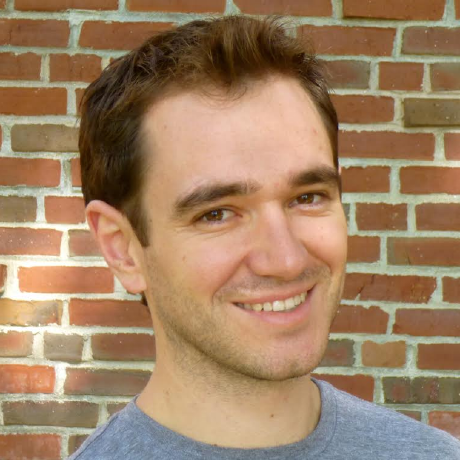
\includegraphics[height=0.16\textwidth]{talkfigs/dougal}
\qquad\qquad
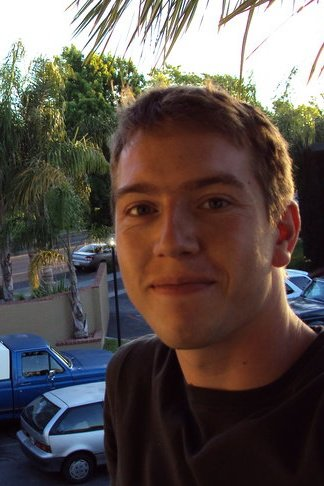
\includegraphics[height=0.16\textwidth, trim=20mm 25mm 0mm 25mm, clip]{talkfigs/david2}
\qquad\qquad
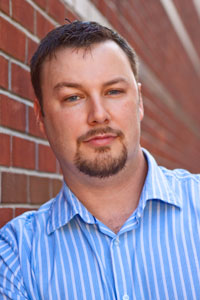
\includegraphics[height=0.16\textwidth]{talkfigs/adams}
\\
Dougal Maclaurin, David Duvenaud, Ryan Adams}

\institute{
\includegraphics[height=0.16\textwidth]{talkfigs/harvard.jpg}}
\date{}

\begin{document}

\frame[plain] {\titlepage}

\frame[plain]{\frametitle{Good ideas always have Bayesian interpretations}
%\begin{itemize}
%\item Regularization -> MAP inference
%\item Dropout -> Integrating over spike-and-slab
%\item Limiting model capacity -> Bayesian Occam's razor
%\item Cross-validation -> Estimating marginal likelihood
%\item Ensembling -> Bayes model averaging?
%\item Early stopping -> ?
%\end{itemize}
\begin{tabular}{rcl}
Regularization & $=$ & MAP inference \\
Limiting model capacity & $=$ &Bayesian Occam's razor \\
Cross-validation & $=$ &Estimating marginal likelihood \\
Dropout        & $=$ &Integrating out spike-and-slab \\
Ensembling & $=$ &Bayes model averaging? \\
Early stopping & $=$ & ??
\end{tabular}
}


\newcommand{\trail}[3]{\includegraphics<#3>[width=6cm]{../experiments/2015_03_02_funnel/5-talk/figures/trails_#1/iter_#2.pdf}}%
\newcommand{\trixa}{0}%
\newcommand{\trixb}{12}%
\newcommand{\trixc}{6}%

\frame[plain]{\frametitle{Gradient descent as a sampler}
\begin{columns}
\hspace{-1cm}\begin{column}{6cm}
\begin{itemize} 
  \item Optimization paths start from random init, and move towards modes...
\end{itemize}
\end{column}
\begin{column}{5cm}
\trail{\trixa}{0}{1}%
\trail{\trixa}{1}{2}%
\trail{\trixa}{2}{3}%
\trail{\trixa}{3}{4}%
\trail{\trixa}{4}{5}%
\trail{\trixa}{5}{6}%
\trail{\trixa}{6}{7}%
\trail{\trixa}{7}{8}%
\trail{\trixa}{8}{9}%
\trail{\trixa}{9}{10}%
\trail{\trixa}{10}{11}%
\trail{\trixb}{0}{12}%
\trail{\trixb}{1}{13}%
\trail{\trixb}{2}{14}%
\trail{\trixb}{3}{15}%
\trail{\trixb}{4}{16}%
\trail{\trixb}{5}{17}%
\trail{\trixb}{6}{18}%
\trail{\trixb}{7}{19}%
\trail{\trixb}{8}{20}%
\trail{\trixb}{9}{21}%
\trail{\trixb}{10}{22}%
\trail{\trixc}{0}{23}%
\trail{\trixc}{1}{24}%
\trail{\trixc}{2}{25}%
\trail{\trixc}{3}{26}%
\trail{\trixc}{4}{27}%
\trail{\trixc}{5}{28}%
\trail{\trixc}{6}{29}%
\trail{\trixc}{7}{30}%
\trail{\trixc}{8}{31}%
\trail{\trixc}{9}{32}%
\trail{\trixc}{10}{33}%
\end{column}
\end{columns}}

\newcommand{\dist}[2]{\includegraphics<#2>[width=6cm]{../experiments/2015_03_02_funnel/6-nicer/figures/dists_#1.pdf}}%

\frame[plain]{\frametitle{Implicit Distributions}
\begin{columns}
\hspace{-1cm}\begin{column}{6cm}
\begin{itemize} 
\item What about the implicit distribution of parameters after optimizing for $t$ steps?
\item Starts as a bad approximation (prior dist)
\item Ends as a bad approximation (point mass)
\item Ensembling $=$ taking multiple samples from dist
\item Early stopping $=$ choosing best intermediate dist
\end{itemize}
\end{column}
\begin{column}{5cm}
\dist{0}{1}%
\dist{1}{2}%
\dist{2}{3}%
\dist{3}{4}%
\dist{4}{5}%
\dist{5}{6}%
\dist{6}{7}%
\dist{7}{8}%
\dist{8}{9}%
\dist{9}{10}%
\dist{10}{11}%
\end{column}
\end{columns}}

\frame[plain]{\frametitle{Cross validation vs. marginal likelihood}
\begin{columns}
\hspace{-1cm}\begin{column}{6cm}
\begin{itemize} 
\item What if we could evaluate marginal likelihood of implicit distribution?
\item Could choose all hypers to maximize marginal likelihood
\item No need for cross-validation?
\end{itemize}
\end{column}
\begin{column}{5cm}
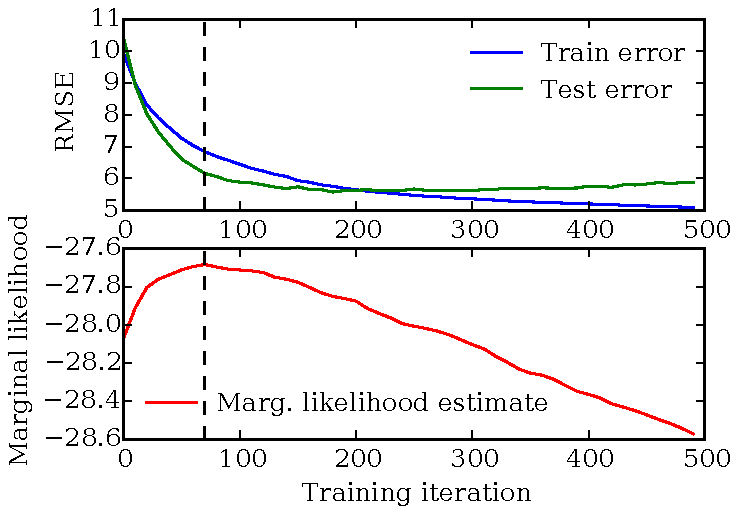
\includegraphics[width=1.15\columnwidth]{../experiments/2015_03_01_housing/2/marglik.pdf}
\end{column}
\end{columns}}

\frame[plain]{\frametitle{Variational Lower Bound}
\begin{align*}
\log p(\data) \geq - \underbrace{\expectargs{q(\params)}{ -\log \jointdist }}_{\textnormal{\normalsize Energy $E[q]$}}
 \quad \underbrace{- \expectargs{q(\params)}{\log q(\params)}}_{\textnormal{\normalsize Entropy $S[q]$}}
%& := \varL[q] \label{eq:varbound}
\end{align*}
Energy estimated from optimized objective function (training loss is NLL):
\begin{align*}
\expectargs{q(\params)}{-\log \jointdist} & \approx - \log p(\hat\theta_T, \vx) %\subjointdist{}{T}
\end{align*}
Entropy estimated by tracking change at each iteration:
\begin{align*}
- \expectargs{q(\params)}{\log q(\params)} & \approx S[q_0] + \sum_{t=0}^{T-1} \log \left| J(\hat\params_t) \right|
\label{eq:entropy-bound}
\end{align*}
Using a single sample!% sometimes OK in high dimensions.
}


\frame[plain]{\frametitle{Estimating change in entropy}
\begin{columns}
\hspace{-1cm}\begin{column}{6cm}
\begin{itemize} 
\item Inuitively: High curvature makes entropy decrease quickly
\item Can measure local curvature with Hessian
\item Approximation good for small step-sizes
\end{itemize}
\end{column}
\begin{column}{5cm}
\dist{0}{1}%
\dist{1}{2}%
\dist{2}{3}%
\dist{3}{4}%
\dist{4}{5}%
\end{column}
\end{columns}}

\frame[plain]{\frametitle{Estimating change in entropy}

Volume change given by Jacobian of optimizer's operator:
\begin{align*}
S[q_{t+1}] - S[q_t] = \expect_{q_t(\params_t)} \left[ \log \Big| J(\params_t) \Big| \right]
\end{align*}

Gradient descent update rule:
\begin{align*}
\params_{t+1} &=
  \params_t - \stepsize \nabla \loss,
\end{align*}

Has Jacobian:
\begin{align*}
J(\params_t) = I - \stepsize \nabla \nabla L(\theta_t)
\end{align*}

Entropy change estimated at a single sample:
\begin{align*}
S[q_{t+1}] - S[q_t] \approx \log \left| I - \stepsize \nabla \nabla L(\theta_t) \right|
\end{align*}

%\end{column}
%\end{columns}
}

\frame[plain]{\frametitle{Final algorithm}
%\hspace{-1cm}%
\Wider[1cm]{
\begin{minipage}[t]{0.49\columnwidth}
\begin{algorithm}[H]
\caption*{Stochastic gradient descent\phantom{py}} 
\begin{algorithmic}[1]
\scriptsize%
	\State {\bfseries input:}
	Weight init scale $\sigma_0$, step size $\stepsize$,
	negative log-likelihood $L(\params, t)$
	\State {\bfseries initialize} $\params_0 \sim \N{0}{\sigma_0 \vI_D}$
	\State \phantom{{\bfseries initialize} $\entropy_{0} = \frac{D}{2} (1 + \log 2 \pi)$}
	\For{$t=1$ {\bfseries to} $T$}
		\State \phantom{$\entropy_{t} = \entropy_{t-1} + \log \left| \vI - \stepsize \nabla \nabla L(\theta_t, t) \right|$}%\Comment{Update entropy}} 
		\State $\params_{t} = \params_{t-1} - \stepsize \gradparams$ % \Comment{Update parameters}	
   \EndFor
   \State \textbf{output} sample $\params_T$, \phantom{entropy estimate $\entropy_T$}
\end{algorithmic}
\end{algorithm}
\end{minipage}
\hfill
\begin{minipage}[t]{0.49\columnwidth}
\begin{algorithm}[H]
\caption*{SGD with entropy estimate} 
\label{alg:neural} 
\begin{algorithmic}[1]
\scriptsize%
\State {\bfseries input:}
	Weight init scale $\sigma_0$, step size $\stepsize$,
	negative log-likelihood $L(\params, t)$
	\State {\bfseries initialize} $\params_0 \sim \N{0}{\sigma_0 \vI_D}$
	\State {\color{myfavblue}{{\bfseries initialize} $\entropy_{0} = \frac{D}{2} (1 + \log 2 \pi) + D \log\sigma_0$}}
	\For{$t=1$ {\bfseries to} $T$}
		\State {\color{myfavblue}$\entropy_{t} = \entropy_{t-1} + \log \left| \vI - \stepsize \nabla \nabla L(\theta_t, t) \right|$} %\Comment{Update entropy} 
		\State $\params_{t} = \params_{t-1} - \stepsize \gradparams$ % \Comment{Update parameters}	
   \EndFor
   \State \textbf{output} sample $\params_T$, \color{myfavblue}{entropy estimate $\entropy_T$}
\end{algorithmic}
\end{algorithm}
\end{minipage}}

\vspace{1cm}
\begin{itemize}
\item Approximate bound: $\log p(\data) \gtrsim -L(\theta_T) + S_T$
\item Determinant is $\mathcal{O}(D^3)$
\item $\mathcal{O}(D)$ Taylor approximation using Hessian-vector products
\item Scales linearly in parameters and dataset size
\end{itemize}}

\frame[plain]{\frametitle{Choosing when to stop}
\begin{columns}
\hspace{-1cm}\begin{column}{6cm}
\begin{itemize} 
\item Neural network on the Boston housing dataset.
\item SGD marginal likelihood estimate gives stopping criterion without a validation set
\end{itemize}
\end{column}
\begin{column}{5cm}
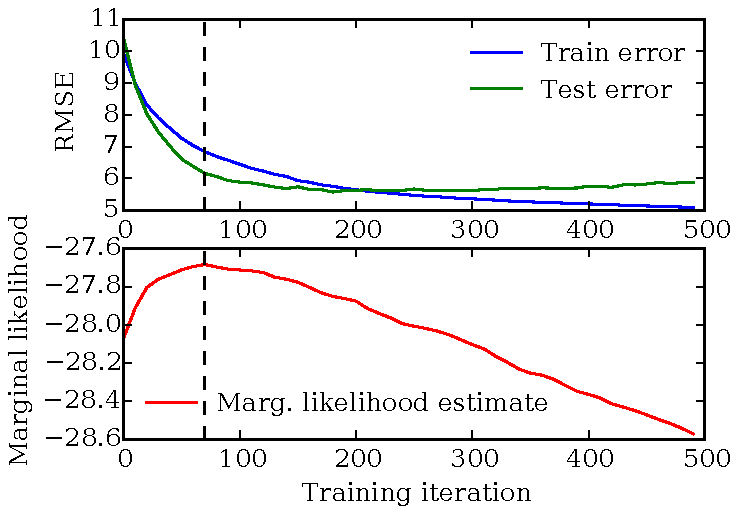
\includegraphics[width=1.15\columnwidth]{../experiments/2015_03_01_housing/2/marglik.pdf}
\end{column}
\end{columns}}

\frame[plain]{\frametitle{Choosing number of hidden units}
\begin{columns}
\hspace{-1cm}\begin{column}{6cm}
\begin{itemize} 
\item Neural net on 50000 MNIST examples
\item Largest model has 2 million parameters
\item Gives reasonable estimates, but cross-validation still better
%\item Inter-sample variance is surprisingly low
\end{itemize}
\end{column}
\begin{column}{5cm}
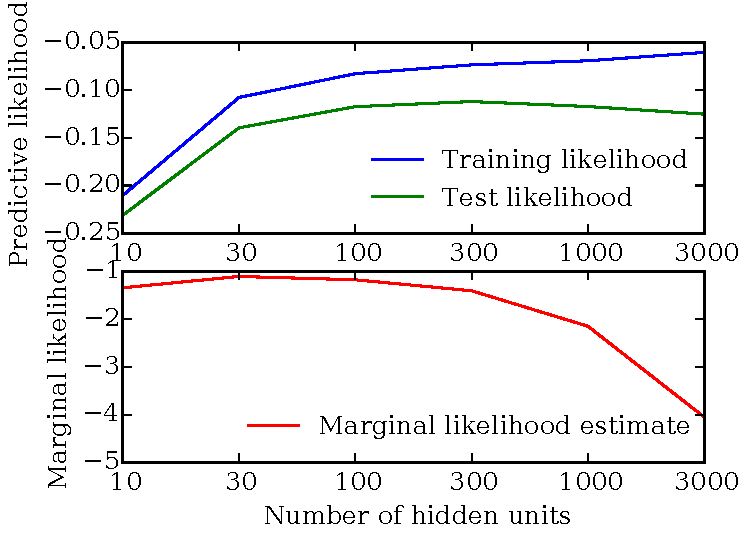
\includegraphics[width=1.15\columnwidth]{../experiments/2015_03_03_vary_width/7_hidden_units_higher_learnrate/vary_widths.pdf}
\end{column}
\end{columns}}

\frame[plain]{\frametitle{Limitations}
\begin{columns}
\hspace{-1cm}\begin{column}{6cm}
\begin{itemize} 
\item SGD not even trying to maximize lower bound -- good approximation is by accident!
\item Entropy term gets arbitrarily bad due to concentration, but true performance only gets as bad as maximum likelihood estimate
\end{itemize}
\end{column}
\begin{column}{5cm}
\dist{3}{1}%
\end{column}
\end{columns}}

\frame[plain]{\frametitle{Entropy-friendly optimization}
\begin{columns}
\hspace{-1cm}\begin{column}{6cm}
\begin{itemize} 
\item Modified SGD to move slower near convergence, optimized new hyperparameter
\item Hurts performance, but gives tighter bound
\item ideally would match test likelihood
\end{itemize}
\end{column}
\begin{column}{5cm}
\includegraphics<1>[width=\columnwidth]{../experiments/2015_03_02_funnel/2/dists.pdf}
\includegraphics<2>[width=\columnwidth]{../experiments/2015_03_02_funnel/3_grad_threshold/dists.pdf}

\hspace*{-0.5cm}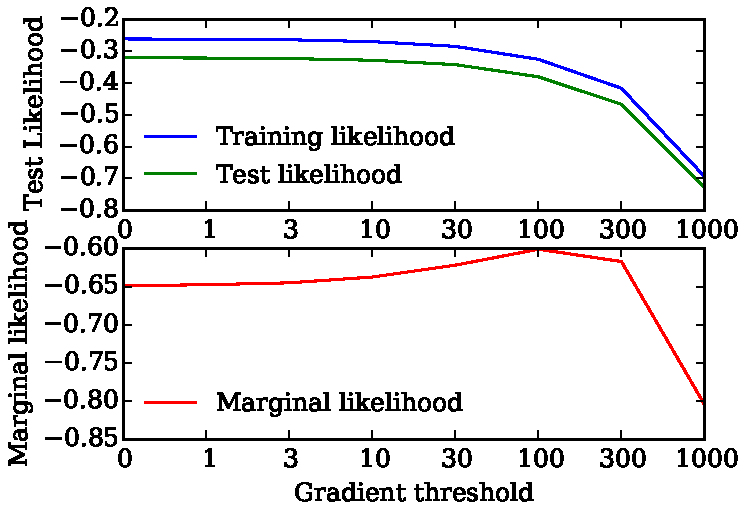
\includegraphics[width=1.15\columnwidth]{../experiments/2015_03_03_vary_width/5_grad_threshold/vary_widths.pdf}
\end{column}
\end{columns}}

\frame[plain]{\frametitle{Limitations}
\begin{columns}
\hspace{-1cm}\begin{column}{6cm}
\begin{itemize}
\item Irrelevant parameters can cause low entropy estimate
\item No momentum - would need to estimate distribution (see Kingma \& Welling, 2015)
\end{itemize}
\end{column}
\begin{column}{5cm}
\dist{3}{1}%
\end{column}
\end{columns}}

\frame[plain]{\frametitle{Main Takeaways}
%\begin{columns}
%\hspace{-1cm}\begin{column}{6cm}
\begin{itemize} 
\item Optimization with random restarts implies nonparametric intermediate distributions
\item Early stopping chooses among these distributions
\item Ensembling samples from them
\item Can scalably estimate variational lower bound on model evidence during optimization
\item Another connection between practice and theory
\end{itemize}
\pause

\centerline{Thanks!}

%\end{column}
%\begin{column}{5cm}
%\end{column}
%\end{columns}
}

\end{document}
